
\documentclass[11pt]{article}
%%%%%%%%%%%%%%%%%%%%%%%%%%%%%%%%%%%%%%%%%%%%%%%%%%%%%%%%%%%%%%%%%%%%%%%%%%%%%%%%%%%%%%%%%%%%%%%%%%%%%%%%%%%%%%%%%%%%%%%%%%%%%%%%%%%%%%%%%%%%%%%%%%%%%%%%%%%%%%%%%%%%%%%%%%%%%%%%%%%%%%%%%%%%%%%%%%%%%%%%%%%%%%%%%%%%%%%%%%%%%%%%%%%%%%%%%%%%%%%%%%%%%%%%%%%%
\usepackage{geometry}
\usepackage{setspace}

%TCIDATA{OutputFilter=LATEX.DLL}
%TCIDATA{Version=5.50.0.2960}
%TCIDATA{<META NAME="SaveForMode" CONTENT="1">}
%TCIDATA{BibliographyScheme=Manual}
%TCIDATA{Created=Tuesday, April 19, 2011 13:53:53}
%TCIDATA{LastRevised=Tuesday, April 30, 2013 22:43:51}
%TCIDATA{<META NAME="GraphicsSave" CONTENT="32">}
%TCIDATA{<META NAME="DocumentShell" CONTENT="Standard LaTeX\Blank - Standard LaTeX Article">}
%TCIDATA{CSTFile=40 LaTeX article.cst}

\newtheorem{theorem}{Theorem}
\newtheorem{acknowledgement}[theorem]{Acknowledgement}
\newtheorem{algorithm}[theorem]{Algorithm}
\newtheorem{axiom}[theorem]{Axiom}
\newtheorem{case}[theorem]{Case}
\newtheorem{claim}[theorem]{Claim}
\newtheorem{conclusion}[theorem]{Conclusion}
\newtheorem{condition}[theorem]{Condition}
\newtheorem{conjecture}[theorem]{Conjecture}
\newtheorem{corollary}[theorem]{Corollary}
\newtheorem{criterion}[theorem]{Criterion}
\newtheorem{definition}[theorem]{Definition}
\newtheorem{example}[theorem]{Example}
\newtheorem{exercise}[theorem]{Exercise}
\newtheorem{lemma}[theorem]{Lemma}
\newtheorem{notation}[theorem]{Notation}
\newtheorem{problem}[theorem]{Problem}
\newtheorem{proposition}[theorem]{Proposition}
\newtheorem{remark}[theorem]{Remark}
\newtheorem{solution}[theorem]{Solution}
\newtheorem{summary}[theorem]{Summary}
\newenvironment{proof}[1][Proof]{\noindent\textbf{#1.} }{\ \rule{0.5em}{0.5em}}
%\input{tcilatex}
\setlength{\parindent}{0in}
\renewcommand{\arraystretch}{.95}
\geometry{left=.8 in,right=.8 in,top=.8 in,bottom=.8 in}

\usepackage{graphicx}
\usepackage{dsfont}
\usepackage{amsmath}
\usepackage{epsfig}
\usepackage{epstopdf}
\usepackage{subfigure}
\usepackage{array}
\newcolumntype{L}[1]{>{\raggedright\let\newline\\\arraybackslash\hspace{0pt}}m{#1}}
\newcolumntype{C}[1]{>{\centering\let\newline\\\arraybackslash\hspace{0pt}}m{#1}}
\newcolumntype{R}[1]{>{\raggedleft\let\newline\\\arraybackslash\hspace{0pt}}m{#1}}
\DeclareMathOperator*{\argmax}{argmax}
\DeclareMathOperator*{\argmin}{argmin}
\usepackage{listings}



\begin{document}

\textbf{Avoided Cost Calculator}

\bigskip

The Avoided Cost Calculator (ACC) is used to determine the primary benefits of distributed energy resources and demand-side programs, such as NEM, across Commission proceedings. 

\bigskip

The Commission approved the first ACC in 2005 with Decision (D.) 05-04-24.  It is designed to estimate the going-forward costs avoided by a DER investment that reduces forecast demand growth over a long (10-30 years) time frame. It is designed to provide ` a straightforward costing methodology that is implemented using a spreadsheet model and publicly available data, resulting in avoided cost estimates that are transparent and can be easily updated to reflect changes in major cost drivers.'  

\bigskip


The output of the model is a set of hourly values over a 30-year time horizon that represents the marginal costs a utility would avoid in any given hour if a distributed energy resource reduced demand for energy during that hour. This emphasis on the reduction of future demand growth  is not perfectly aligned with our application, as we are emphasizing a retrospective look at variable costs incurred to meet realized demand. Another complication is that the E3 ACC methodology/modeling changes year-to-year (especially wrt GHG costs) and there is a 5 year period over which the ACC was not updated. This will complicate the comparisons across years.  


\bigskip

%In some respects, the  IOU general rate cases (GRCs) provide a better approximation to what we want. GRC 2 determines the share of utility costs that each customer class is responsible for (or `causes').  Each large electric utility files a GRC2 application every three years.  Identifying the ways in which these GRC2 cases deviate from E3 ACC methods could be a useful way to think about how we might want to modify the ACC numbers for our purposes. In many 

\bigskip



\section{Definitions}

The ACC calculates six types of avoided costs: generation capacity, energy, transmission and distribution capacity, ancillary services, renewable portfolio standard, and greenhouse gas emissions. The figures below show the relative importance of the key cost components (using 2016 and 2020 ACC calculators).

\bigskip

 \caption{2016 E3 ACC  1 year time horizon} \\
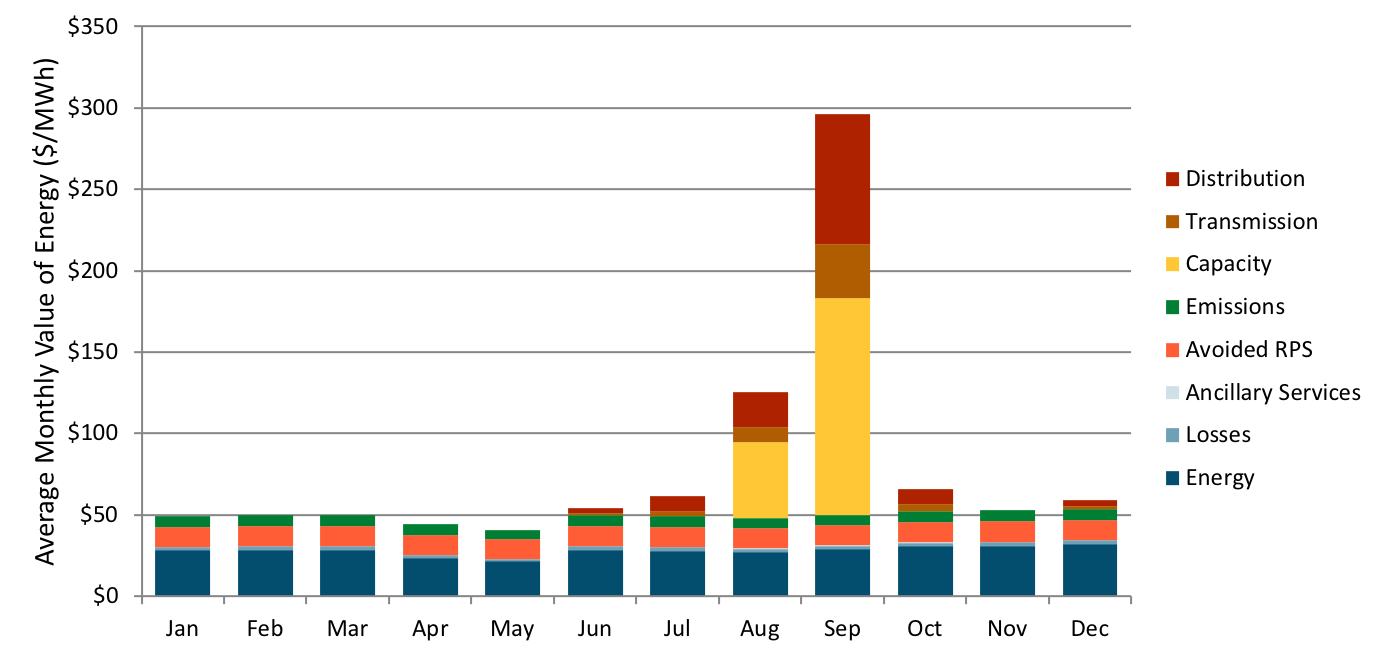
\includegraphics[scale=0.7]{ACC2016.png}


\bigskip

 \caption{2020 E3 ACC  1 year time horizon} \\
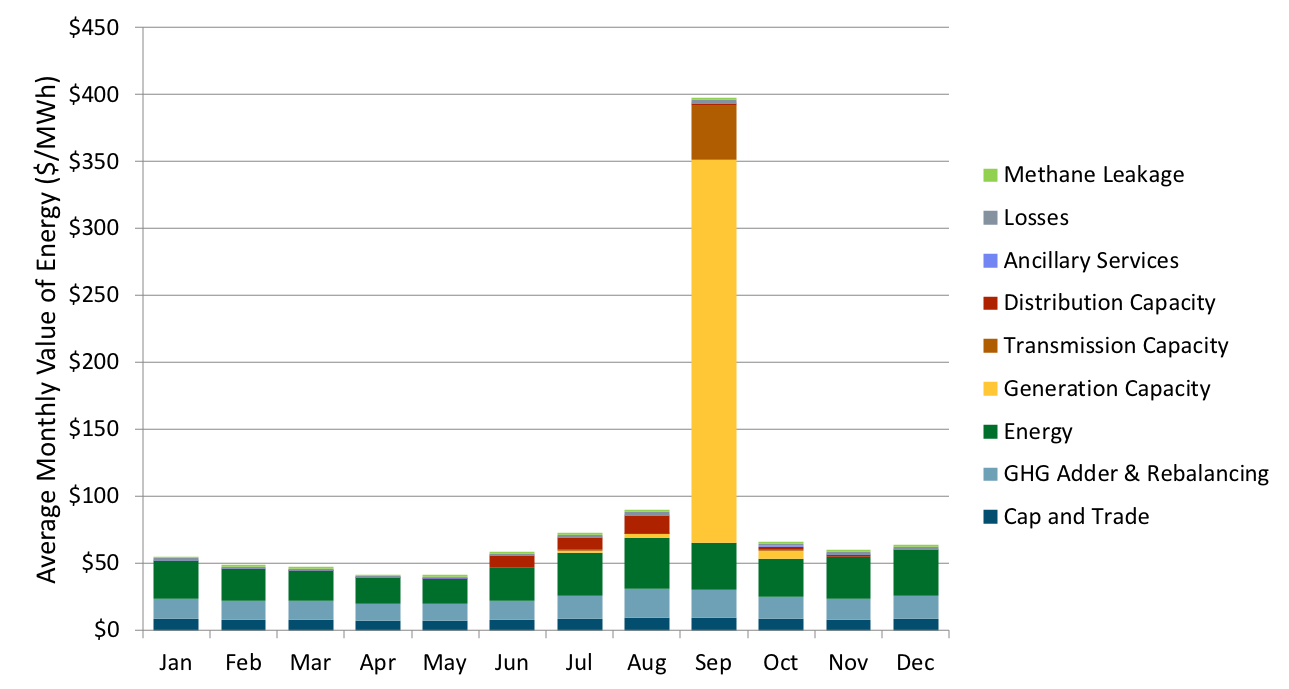
\includegraphics[scale=0.75]{ACC2020.png}


The primary cost components are summarized below:

\subsection{Marginal Energy Cost (MEC)}

The MEC is intended to reflect the cost of procuring electricity to meet one additional megawatt-hour (MWh) of load, measured in cents per kilowatt-hour.  Because the IOUs meet residual needs by purchasing power in the CAISO day-ahead market, ISO wholesale energy price forecasts can be used to estimate the MEC. The E3 ACC generation energy costs are calculated hourly for 16 climate zones. The average energy cost in the near term is based on the OTC Global Holdings Forwards on-peak and off-peak market price forecasts for NP-15 and SP-15, averaged to calculate the system value. Hourly shape is derived from day-ahead LMPs at load-aggregation points in northern and southern California obtained from the California ISO’s MRTU OASIS. 

\bigskip

For the period after the available forward market prices, the method interpolates between the last available futures market price and the long-run energy market price.  E3 has started to use production simulation models (PLEXOS, SERVM) versus ISO forecast prices to estimate this MEC component far into the future. Not so relevant for us if we  work within the window where forecasts are available. 

\bigskip
	
The E3 treatment of generation avoided costs was updated in 2016 to adjust for carbon prices in the electricity market price forecasts. The prior years E3 ACC does not account for this. The updated methodology starts with market prices that include CO2 costs, and decomposes the market price into an energy component and a CO2 component based on the 2015 IEPR CO2 prices and the inferred market heat rates.


\bigskip

I see two problems with using the E3 ACC to construct the energy cost comopnents:

\begin{itemize}
\item  Over the 2010-2015 gap, the E3 ACC uses natural gas forecasts that diverge significantly from realized prices. 
\item  Over 2012-2016, carbon prices are not removed.

\end{itemize}

For this reason, I propose we do the following:

\begin{center}
\begin{equation*}
MEC_{it} = (LMP_{it}-\tau_t \cdot MOER_t )(\frac{1}{1-dL/dQ} )
\end{equation*}
\end{center}

\begin{itemize}

\item Adjust for line losses. Use the $\frac{1}{1-dL/dQ}$ estimates from SMC2. These are differntiated by utility hour. 
\item Adjust for permit costs $\tau_t  \cdot MOER_t$

\end{itemize}

GHG permit prices. We could use auction prices. 

\bigskip

We also need hourly MOER estimates. E3 GHG impacts are based on hourly marginal emissions, calculated using an implied heat rate methodology that incorporates market price forecasts for electricity and natural gas, as well as gas generator operational characteristics. This process assumes that natural gas is the marginal fuel in all hours. The hourly emissions rate of the marginal generator is calculated based on the day-ahead market price curve (with the assumption that the price curve also includes the cost of CO2):
\begin{center}
\begin{equation*}
HeatRate_{t} = (LMP_t  - VOM) / (GasPrice_t + EF * \tau_t)
\end{equation*}
\end{center}
Where:

\begin{itemize}
\item LMP is the hourly market price of energy. 
\item VOM is the variable O&M cost for a natural gas plant.  This is included in the E3 ACC documentation.
\item GasPrice is the cost of natural gas delivered to an electric generator. We can get this from EIA? SNL?
\item $\tau$ is the \$/ton cost of CO2. 
\item EF is the emission factor for tons of CO2 per MMBTU of natural gas. E3 assumes 0.0585 tons/MMBtu. 
\end{itemize}

The link between higher market prices and higher emissions rates is intuitive: higher market prices enable lower-efficiency generators to operate, resulting in increased rates of emissions at the margin. Of course, this relationship breaks when gas is not on the margin. For this reason, the avoided cost methodology bounds the maximum emissions rates based on the range of heat rates of gas turbine technologies ( 0 - 12,500 btu/kWh).

\bigskip

To cross-check can compare our numbers to those reported by E3 for the years we have.


\subsection{GHG component}

Conceptually, the E3 GHG cost is comprised of two components: the monetized allowance value embedded in the energy price and the non-monetized carbon price in excess of the allowance value. The 2020 ACC adds an additional `rebalancing' step described below (one we do not want to take/adopt)

\bigskip
 
I think we should just use the MOERs we estimate in the prior step and multiply by the SCC. 

\bigskip
 
Note that the E3 ACC also estimates marginal emissions rates for local pollution. We could add these in using EPA estimates of the costs per ton of NOx and SO2. These will be small.  


\subsection{Marginal Generation Capacity Costs (MGCC)}

The MGCC captures the fixed cost of procuring and operating generation capacity to meet one additional megawatt of peak load. These are measured in terms of  dollars per kilowatt-year.  There are some important differences in how E3 ACC generation capacity costs are computed in 2010 versus 2016:

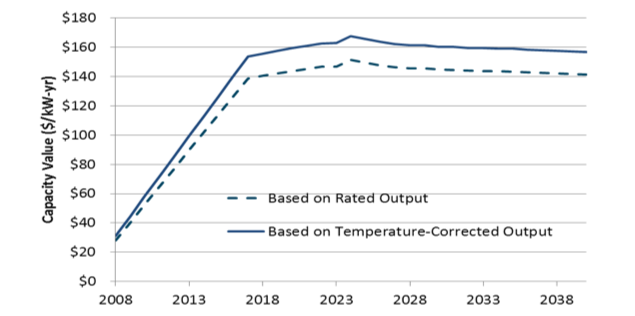
\includegraphics[scale=1]{MGC_11.png}\\


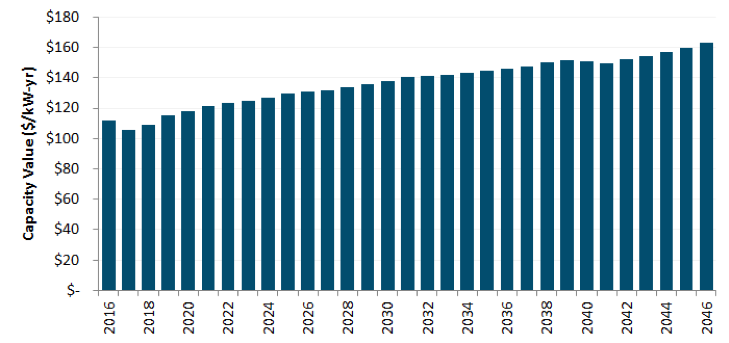
\includegraphics[scale=1]{MGC16.png}\\

Some background and context:

\begin{itemize}

\item The resource balance year is defined as “the year in which new forecasts predict new capacity will be needed; i.e., the year that generation resources are no longer balanced with load”. 

\item In the 2010 ACC, the resource balance year was defined to be 2017. The 2008 resource adequacy value was estimated \$28.07/kW.  The graph above suggests that the ACC model interpolates between this 2008 RA value and the residual capacity value that kicks in at the resource balance year.

\item The 2016 E3 ACC documentation refers to a “May 3, 2016 Proposed Decision of Commissioner Florio in R. 14-10-003 has essentially set the Resource Balance Year to zero, which means E3 now uses the long-run capacity cost for all years.”  I cannot find this language in the Florio decision. 

\item After the resource balance year, the generation capacity cost is the levelized capital cost of a new simple cycle CT unit less the margin that the CT could earn from the energy and ancillary service markets. In 2016, this calculation updated to include carbon costs in both the bid prices for the CT and the market prices for energy.

\item To determine the long-run value of capacity, the avoided cost model performs an hourly dispatch of a new CT to determine energy market net revenues. The CT’s net margin is calculated assuming that the unit dispatches at full capacity in each hour that the real-time price exceeds its operating cost (the sum of fuel costs and variable O&M) plus a bid adder of 10\%.  In each hour that it operates, the unit earns the difference between the market price and its operating costs.  

\item The market revenues earned in the energy and AS markets are subtracted from the fixed and variable costs of operating a CT to determine the residual capacity value.   One thing to note is that E3 natural gas price forecasts are on the high side. This will drive up wholesale price forecasts and thus reduce residual capacity value. 

\item In 2020, to create greater alignment with IRP, the generation capacity value will now use a new 4-hour
battery storage resource as a proxy. 


\end{itemize}


How to allocate these capacity costs across hours?

\begin{itemize}

\item 	In the 2010 E3 ACC, residual capacity value is allocated across the top 250 hours of CAISO system load, in inverse proportion to the gap between the system peak load plus operating reserves and the system loads for each of the 250 hours.  Note that capacity value allocated across these 250 hours even if generation capacity constraints do not bind!

\item 	In this manner, the highest load hour will receive the largest allocation of capacity value on a \$/kWh basis (~\$2,000/MWh). The 250th hour receives an allocation of ~\$400/MWh.  Most of the capacity value falls in the summer on-peak period, though some falls in the summer and winter partial-peak periods as well.    

\item 	2016 updated the approach to allocating residual capacity value uses the “RECAP” model that generates hourly, system wide expected unserved energy (EUE) values.  The residual  capacity values (\$/kW-yr), after adjusting for temperature, losses, and planning reserve margin, are then allocated to the hours of the year with highest system capacity need using the E3 RECAP model. Documentation does note the problem that arises when all hours have 0 EUE!

\item GRCs take a similar weighting approach based on the likelihood that the electric system will be unable to serve customer demand in any given hour. There is always some likelihood, however small, that the system will be unable to serve demand due to insufficient availability of generation relative to the electricity demanded by customers. The risk of a generation shortage can be reduced by having more generation available than forecast peak demand (i.e., a reserve margin), but this additional generation capacity imposes costs on customers. Loss of Load Expectation (LOLE) is a measure that predicts the ability (or inability) to deliver energy to the load. An LOLE analysis can provide insight into the planning reserve margin required for each LSE in a region. The relative LOLE provides a method for allocating annualized capacity 22 value across hours in proportion to when the loss of load. 

\end{itemize}

I propose we do the following:


\textbf{OPTION 1}: Use E3 ACC GCC off the shelf.  I believe we can extract from the ACC the IOU specific capacity values in each ACC year. We can interpolate across the missing years between 2010 and 2016. We can then assign these values to years using the PCAF formula. That is, take the top 250 hours and estimate the following:

\begin{equation*}
PCAF_h =  ( Peak load - Load_h) / \sum_h (Peak-Load_h)
\end{equation*}

We should double check that this comes pretty close to replicating the ACC hourly GCCs.

\textbf{OPTION 2}: RA approach? 

Use the same PCAF weights to allocate a short run capacity cost of \$30/kW-yr.

\begin{itemize}

\item 	In the 2016 GRC, PG&E estimated the short-run cost of capacity as the going-forward fixed cost of the existing generation resource net of energy gross margins it earns from the spot energy market over the period  2017-2022.  They assumed an existing combined cycle gas turbine (CCGT) plant as the marginal unit. The going-forward fixed cost consists of fixed O&M, insurance and property tax. Insurance and property tax are estimated based on the capital costs.  

\item 	To calculate levelized MGCC, PG&E first calculated a Net Present Value (NPV) sum of the six years of MGCCs and then converted this NPV to a levelized value. PG&E used its after-tax Weighted Average Cost of Capital (WACC) of 7.0 percent. The estimated net costs of capacity:  \$30.23/kW-year, \$29.62/kW-yr, \$28.53/kW-yr, \$27.63/kW-yr, \$27.70/kW-yr and \$27.42/kW-yr for 2017 through 2022, respectively. 

\item 	This represents the cost of an existing CCGTs fixed costs above and beyond what it could earn in the energy market. These are much closer to the resource adequacy value that E3 estimated at \$28.07/kW. 

\end{itemize}


\subsection{Marginal Transmission Capacity Costs (MTCC) }


Transmission avoided capacity costs represent the potential cost impacts on utility transmission investments from changes in peak loadings on the utility systems. The paradigm is that reductions in peak loadings via customer demand reductions, distributed generation, or storage could reduce the need for some transmission projects and allow for deferral or avoidance of those projects. The ability to defer or avoid transmission projects would depend on multiple factors, such as the ability to obtain sufficient dependable aggregate peak reductions in time to allow prudent deferral or avoidance of the project, as well as the location of those peak reductions in the correct areas within the system to provide the necessary reductions in network flows.

\bigskip

On a regular basis, IOUs coordinate with the California Independent System Operator (CAISO) to plan transmission expansion upgrades (5 to 10 year time frame). If a given facility loading is reduced considerably prior to the implementation date, due to demand forecasts, then the implementation date of a planned transmission project may be deferred. Deferrable transmission projects are thus defined as  `demand-related' marginal  transmission investments. If a project is deemed to be `deferrable', this means that the  project is driven by demand, and not by regulatory, safety, contractual, efficiency or other reasons. 


\begin{itemize}


\item In the E3 ACC, marginal transmission capacity costs are based on these deferrable transmission projects. They represent the potential cost impacts on utility transmission investment from changes in peak loadings.

\item As PG&E is the only utility to file transmission-level costs in their general rate case, earlier versions of the ACC has included avoided future transmission costs for PG&E but not for SCE or SDG&E. 


\item PG&E has estimated those values for ratemaking purposes using the Discounted Total Investment Method (DTIM). The DTIM calculates the unit cost of transmission capacity as the present value of peak demand driven transmission investments divided by the present value of the peak demand growth.  This unit cost is then annualized using a Real Economic Carrying Charge (RECC) with adjustments for other ratepayer-borne costs, such as administrative and general costs (A&G) and operations and maintenance costs (O&M).  

\item Several stakeholders (e.g. Clean Coalition) argued successfully to extend this approach to other utilities in 2020.


\item Other stakeholders offer a different view. For example, CLECA argues that most	current	and	new	transmission	investment	is	not	driven	by 	load	growth	and	is	not	marginal (cite	CAISO	e.g.	2016-2017	TPP	at	102- 104).

\item CERCLA submitted data requests to prove this point. 

\begin{itemize}

\item For	SCE,	 only	2-4\%	of	its	forecast	transmission	 system	 cap	ex	is	load-growth	related. The	rest	is	for	RPS,	reliability,	and	grid	operations	needs.  The	result	is	low	marginal	transmission	capacity	costs.

\item For	PG&E,	a	response	to	a	CLECA	data	request 	in	its GRC	Phase	2	shows	a	MTCC	of	\$3.93/kW- year. 

\item For	SCE,	a	response	to	a	CLECA	data	request	in	its	 GRC	Phase	2	shows	a	MTCC	of	\$21.40/kW- year	

\end{itemize}

\item These numbers are much smaller than E3 estimates. Data	do 	not	support	claims	that	there	are	large	marginal	or	avoidable	 transmission	costs. 

\end{itemize}

Upshot. \$0 is probably too small. 


\subsection{Marginal Distribution Capacity Costs (MDCC)}


The Avoided Cost Calculator has a single avoided distribution value in each of the Southern California Edison Company (SCE) and San Diego Gas & Electric Company (SDG&E) territories based on the marginal cost of distribution from the general rate case. The Pacific Gas and Electric Company (PG&E) avoided cost of distribution value is also based on the marginal cost of distribution from the general rate case and is further broken out by climate zone. 

\bigskip

Unspecified distribution deferral avoided costs reflect the cost of distribution capacity projects that are likely to be needed in the future but are not specifically identified in current utility distribution planning. 


\begin{itemize}

%\item MDCC values are used for marginal cost revenue calculations and rate design, avoided cost modeling, among other things. 

%\item PG&E’s distribution system is defined as facilities operated at voltages less than 50 kilovolts (kV). The system is further divided into primary distribution system (>4V); and  the secondary distribution system. 

\item A detailed planning process uses uses peak load data and load growth forecasts to evaluate whether existing substation and feeder capacity is sufficient so that equipment is not overloaded and so that  service-operating parameters (e.g., voltage limits and adequate reliability levels) are maintained under both normal, and emergency operating conditions.

\item As a general rule, the costs of operating, maintaining and replacing distribution equipment, once installed, are independent of usage. Such costs associated with existing distribution equipment are properly considered fixed costs and excluded from marginal cost calculations.

\item However, there are two types of investments that are made to meet demand growth: (1) Distribution reinforcement investments provide capacity  to meet demand growth on the existing system and (2) distribution investments for primary line extensions provide access and the associated capacity for new demand due to the addition of new customers. 

%\item PG&E estimates MDCC values for three subcomponents: (1) marginal primary distribution capacity costs;  (2) marginal primary distribution capacity costs for new business; and (3) marginal secondary distribution capacity costs. 

\item Primary distribution marginal costs are reported  in dollars per PCAF-kilowatt (kW) per year and primary distribution for new  business and secondary distribution marginal costs are shown in dollars per FLT-kW per year.  

\item In the ACC, these marginal costs are allocated across hours using distribution Peak Capacity Allocation Factors (PCAF). 

\end{itemize}


%In its discussion of the challenges associated with developing an avoided transmission and distribution methodology, the staff concluded that the assessment of the uncertainty associated with each type of deferral value pointed to the appropriate level of precision and disaggregation of the analysis use for the use case.


\bigskip

Many parties have amply documented why no value should be incorporated into the ACC for avoided distribution  costs. 

\begin{itemize}

\item Public Advocates Office recommends a zero value for unspecified avoided distribution costs `because any non-zero value  is likely to be uncertain and inaccurate; rather, a zero value for avoided distribution costs would align with the findings of the
Distributed Resources Planning (“DRP”) Staff Paper on unspecified distribution deferral value.23'

\item TURN argues that it is erroneous to assume that DERs could defer distribution upgrades which are intended to repair equipment or harden the grid to prevent utility-caused ignitions. 

\item CLECA argues that the use of GRC marginal costs for unspecified distribution benefits could lead to over-estimation of the true benefits.

\end{itemize[

Not only is no clear record evidence available that DERs are capable of deferring transmission costs, DERs may increase congestion problems in certain areas



\end{document}

\section{Avoided cost details}

\subsection{MEC}

\begin{itemize}

\item  In past GRC filings,  PG&E forecasts hourly prices  over a 6 year time horizon based on historical day-ahead prices. The MEC for each of PG&E’s six TOU periods is estimated as the average of the hourly electricity price forecasts weighted by the hourly 2014 PG&E system loads (time-shifted so that weekends line up between hourly prices and hourly loads).

\item In contrast, SCE uses an internal PLEXOS production simulation model to forecast ISO market clearing prices over a 3 year period for GRC filing.

\item Prior to 2020, E3 near-term energy costs were based on on-peak and off-peak market forecasts when available.
For the periods farther into the future, they interpolate between the latest available forward price and the long-run energy market price (set so that a CCGT energy market revenues \textit{plus the capacity market payments} equals fixed and variable cost plus carbon costs).

%\item \textbf{Confusion \#1} I am confused about the long  interactions between simulated long run energy price and assumptions about capacity prices? And I am confused how short and long term prices are weighted in their MEC measures.

%\item Hourly shaping: They convert annual energy avoided cost to hourly values using 8760 `market shapes' derived from LMPs at NP15 and SP15. 


\item  The 2020 E3 ACC has moved to using production simulation do develop energy values for the ACC. Use a  production simulation model (SERVM).   Market prices reported directly from SERVM include the effects of carbon pricing from the cap and trade market. In post-processing the SERVM prices, the cap and trade value is backed out to provide an hourly energy only value for use in the ACC. The remaining energy value includes only fuel costs and power plant operating costs.

\end{itemize}

\textbf{Comment}: Differences in methods seem most significant far into the future. We should be setting the time frame to one year, correct?

\textbf{Question}: One methodological difference across sources/years: treatment of GHG permit value. How do we want to deal with this component?


\subsection{GHG costs}

\begin{itemize}

\item In earlier ACC calculations, the GHG costs were based on changes in GHG output of the marginal generating unit in each hour of the year (i.e. the marginal operating emissions rate). 

\item In 2018, E3  GHG values reflected both the monetized GHG permit cost embedded in energy prices and the non-monetized GHG value beyond the permit price.

\item Recent methodological changes (2020) respond to the fact that a DER investment will impact future emissions as the system is rebalanced to reflect new levels of consumption and emissions. Whereas earlier analyses took GHG emissions as given, the most recent (2020) argues that this is not reasonable with increasing electrification.  I found the calculation on page 27 confusing. But the idea is to `rebalance' so that emissions intensity (versus emissions) is exogenously determined.  

\item In the case of a load reduction, rebalancing will reduce the avoided GHG benefits. The figure below turns off rebalancing (and you can see the  GHG adder is larger). 

\end{itemize}

\texbf{Comment} Playing around with the 2020 calculator, rebalancing has a non-negligible impact on a one year forecast.  This effect seems too big... ask E3 about this?




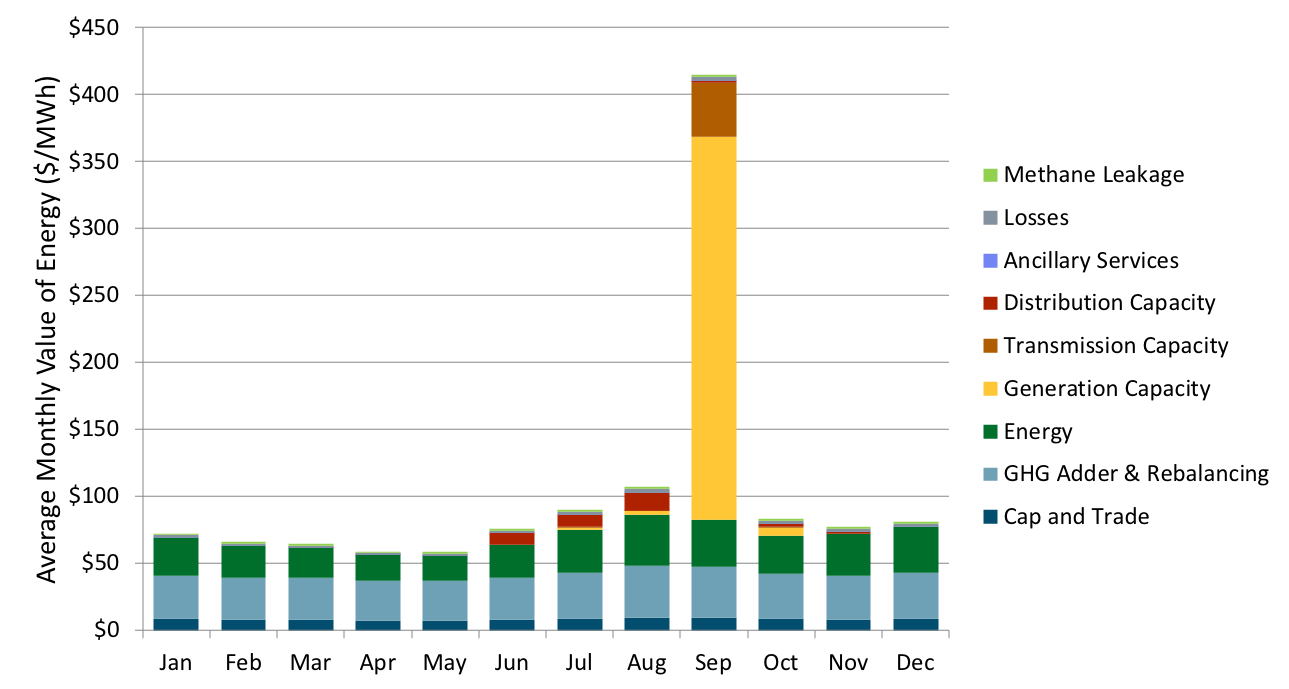
\includegraphics[scale=0.7]{ACC2020nobalance.png}

\textbf{Question} How do we want to deal w GHG costs for our purposes?

\subsection{MGCC}

\begin{itemize}

\item In the 2016 GRC, PG&E estimated the short-run cost of capacity as the going-forward fixed cost of the existing generation resource net of energy gross margins it earns from the spot energy market over the period  2017-2022.  They assumed an existing combined cycle gas turbine (CCGT) plant as the marginal unit. The going-forward fixed cost consists of fixed O&M, insurance and property tax. Insurance and property tax are estimated based on the capital costs.  Notably, this is not a `growth-driven' cost.


\item  PG&E estimated net costs of capacity:  \$30.23/kW-year, \$29.62/kW-yr, \$28.53/kW-yr, \$27.63/kW-yr, \$27.70/kW-yr and \$27.42/kW-yr for 2017 through 2022, respectively. This represents the cost of an existing CCGT’s fixed costs above and beyond what it could earn in the energy market


\item To calculate levelized MGCC, PG&E first calculated a Net Present Value (NPV) sum of the six years of MGCCs and then converted this NPV to a levelized value using the same discount rate. PG&E used its after-tax Weighted Average Cost of Capital (WACC) of 7.0 percent. The resulting levelized MGCC is \$28.64/kW-year. This is much lower than the E3 ACC .... I think because it is not the cost of building new capacity to meet increasing peak, it's the fixed cost of meeting current peak. 

\item In a final step, a weighted portion of demand related costs is assigned to every hour in excess of 80\% of peak demand.  This PCAF calibration proceeds in three steps:

\begin{enumerate}

\item Identify the PCAF hours: Generation PCAF hours are defined as hours during which the total system load is above 80 percent of the system maximum load during the calendar year. 

\item For each identified PCAF hour, the corresponding PCAF weight is constructed such that the peak hour has an allocation that is 20 times the allocation for the hours at 81\% of peak demand and twice the allocation of an hour at 90\% of peak demand.

\item Using customer class net metered loads, calculate
PCAF-weighted loads for each customer class.

\end{enumerate}
\end{itemize}


\textbf{Stupid question}:  If we allocate MGCC costs to *hours*  using this PCAF factor, does this guarantee that revenues earned over and above variable costs equal the levelized MGCC to be recovered in expectation? 


\item Prior to 2020, E3 estimates the levelized capital cost of a new CCGT  unit less the margin the plant would earn on the energy and ancillary service markets (including carbon costs)

\item The 2020 ACC calculates the Net Cost of New Entry (CONE) of a new battery storage resource instead of a gas combustion turbine.

\item Start with the capital cost and subtract simulated market revenues from energy and AS markets. Allocate these residual  capacity costs across hours of the year using the E3 RECAP model ``which determines the expected unserved energy for each month/hour/day.'' This all assumes there will be a need for new capacity going forward.

\item \textbf{Point of confusion number 1:} Whereas IOUs  focus on going forward fixed operating costs, E3 focusing on new investment costs (CCGT or storage). E3 2018 MGCC estimates much higher than PG&E estimates. If load is not growing in a given year, shouldn't MGCC be limited to fixed operations versus new investments cotss?


\item \textbf{Point of confusion number 2:} Minor issue- Are there important differences between the EUE and values and the PCAF approach?


\end{itemize}


\subsection{MTCC}

\begin{itemize}

\item IOU-specific forward-looking MTCCs are estimated using the Discounted Total Investment Method (DTIM).

\begin{enumerate}

\item Calculate the marginal investment per megawatt (MW) as the present value of deferrable investments divided by the present value of forecast load growth. The result is the marginal investment per MW. 


\item This unit cost is then annualized  using a Real Economic Carrying Charge (RECC) factor. The resulting marginal cost ( dollars per MW per year) reflects the annualized cost of investment as well as other capital costs and annual expenses associated with adding capacity to the transmission system. 

\end{enumerate}


\item Note that the RECC takes the investment cost and reshapes them to reflect a stream of costs that increases with inflation and has the same present value as the revenue requirements. Inputs to a RECC: the capital structure and cost of capital, a discount rate, income tax parameters, book depreciable life and costs of
property taxes and insurance. 



\item \item E3 obtains the values used to support GRC cases to estimate their transmission cost components.  For example:

\begin{enumerate}
\item PG&E estimate demand-driven investment of \$200,000,000.
\item Forecast load growth of 1800 MW.

\item This works out to \$111,111  /MW (or \$111/kW).

\item The RECC factor is 11\%. So the marginal transmission capacity cost is\$12.22/kW-year.

\end{enumerate}


\item Notably,  this approach generates non-sensical results during periods of negative load growth. On page 41 of the 2020 E3 ACC documentation with reference to SDGE: `` Unfortunately, the provided system peak load data reflected a negative load growth trend. With that negative growth trend, the method resulted in a nonsensical negative marginal capacity cost for transmission''.   So they smooth growth over years. This raises the question of what to do in years where capacity constraints don't bind?

\end{itemize}

\subsection{MDCC}

\begin{itemize}

\item IOU-specific forward-looking MDCCs are estimated using the Discounted Total Investment Method (DTIM).


\begin{enumerate} 

\item  Calculate the present value for a stream of capacity-related  investments and divide that present value amount by the present value of the corresponding forecast load growth (in kW): the result is a marginal investment cost for a kW change in capacity.  The forecasted investment for large projects and  forecasted capacity growth  are provided by the IOUs. These large  projects generally cause marginal cost “lumpiness” over both geographic and time dimensions.
 
\item Calculate an annualized marginal cost in dollars per MW per year using a Real Economic Carrying Charge (RECC) factor. The resulting marginal cost reflects the annualized cost of investment as well as other capital costs and annual expenses associated with adding capacity to the transmission system. 


\end{enumerate}



\item Note that the RECC takes the investment cost and reshapes them to reflect a stream of costs that increases with inflation and has the same present value as the revenue requirements. Inputs to a RECC: the capital structure and cost of capital, a discount rate, income tax parameters, book depreciable life and costs of
property taxes and insurance. 


\item The Commission has indicated that marginal costs should “reflect geographic differences where significant.” 
PG&E, for example, has a wide variation in the marginal cost of distribution capacity among the more than 240 DPAs that comprise its electric system. Accordingly, PG&E  estimates marginal costs by DPA, and then aggregates those costs into PG&E’s operating divisions.



\item The 2017 PG&E rate filing lists MDCC results for each division (Table 6-1). This is similar to- but different from- the numbers used by the E3 ACC.  They use 2014 GRC numbers (Table 4)  which are mostly (but not all) higher.

\item Similarly, the distribution costs assumed by the ACC are taken from a 2015 GRC and are higher than those reported in the 2018 GRC.

\item The E3 ACC allocates these T&D capacity costs to hours using a regression model that predicts hourly distribution demand as a function of temperature, HDD, CDD, hour and month FE. They then subtract off forecast PV penetration.

\item They simulate distribution loads using 2017 weather data for each climate zone.   They then compare these simulated hourly load against these climate zone specific thresholds (defined as the area maximum demand less one standard deviation??) : $(Load[a,h]-Threshold[a])$.

\item They normalize these by the sum of all positive differences to estimate peak capacity allocation factors (PCAF) for each climate zone and hour.  Intuitively, if  we sum across *all* kWh charged this capacity cost (not just residential), should we recover the reported annualized marginal cost per unit of capacity? 

\end{itemize}
\end{document}


